\documentclass[a4paper]{article}
\usepackage{color}
\usepackage{url}
\usepackage[T2A]{fontenc} 
\usepackage[utf8]{inputenc} 
\usepackage{graphicx}
\usepackage[english,serbianc]{babel}
\usepackage[unicode]{hyperref}
\usepackage{graphicx}
\graphicspath{{./slike/}}
\hypersetup{colorlinks,citecolor=green,filecolor=green,linkcolor=blue,urlcolor=blue}


\begin{document}
	\title{Сајбер криминал и мере заштите\\ \small{Семинарски рад у оквиру курса Техничко и научно писање\\ Математички факултет}}
	
	\author{Богдан Мицић\\ bogdanmicic03vr@gmail.com\\ Никола Милорадовић\\ nikolamiloradovic456@gmail.com\\ Филип Антанасковић\\ filipantana@gmail.com\\ Исидора Перовић\\ dojaperovic@gmail.com} 
	\maketitle
	\abstract{
		Огроман развој технологије је узроковао и развој сајбер (енг. cyber) криминала. Како је технологија све више присутнија у нашим животима, ми као појединци и компаније бивају угроженије од сајбер напада. Овај текст треба проширити свест о сајбер криминалу и његовој претњи као и начине како се боримо против њега и како се може заштити од њега.
	}
	\tableofcontents
	\newpage
	
	\section{Увод : О сајбер криминалу и дигиталној форензици}
         \label{sec:Uvod}
        Са појавом рачунара и рачунарских мрежа, њиховом експанзијом и интеграцијом у свакодневни живот, упоредо долази и до развоја разних метода за њихову експлоатацију и злоупотребу.

        Разлози за ту појаву су различити. На првом месту разлог је стицање финансијске добити. Као други мотиви за нападе на рачунарске системе истичу се 
        изазов, знатижеља, крађа података, шпијунажа и други. Једно од чешћих сајбер криминалних дела је скидање и коришћење "пиратских" програма или мултимедијалних садржаја; односно, садржаја који би легално требало да буду купљени како бисмо их користили, али који се ставе на одређене сајтове преко којих корисници могу да их преузму бесплатно.

        На слици 1 приказано је коришћење интернета током година:

        \begin{figure}[h]
        \centering
        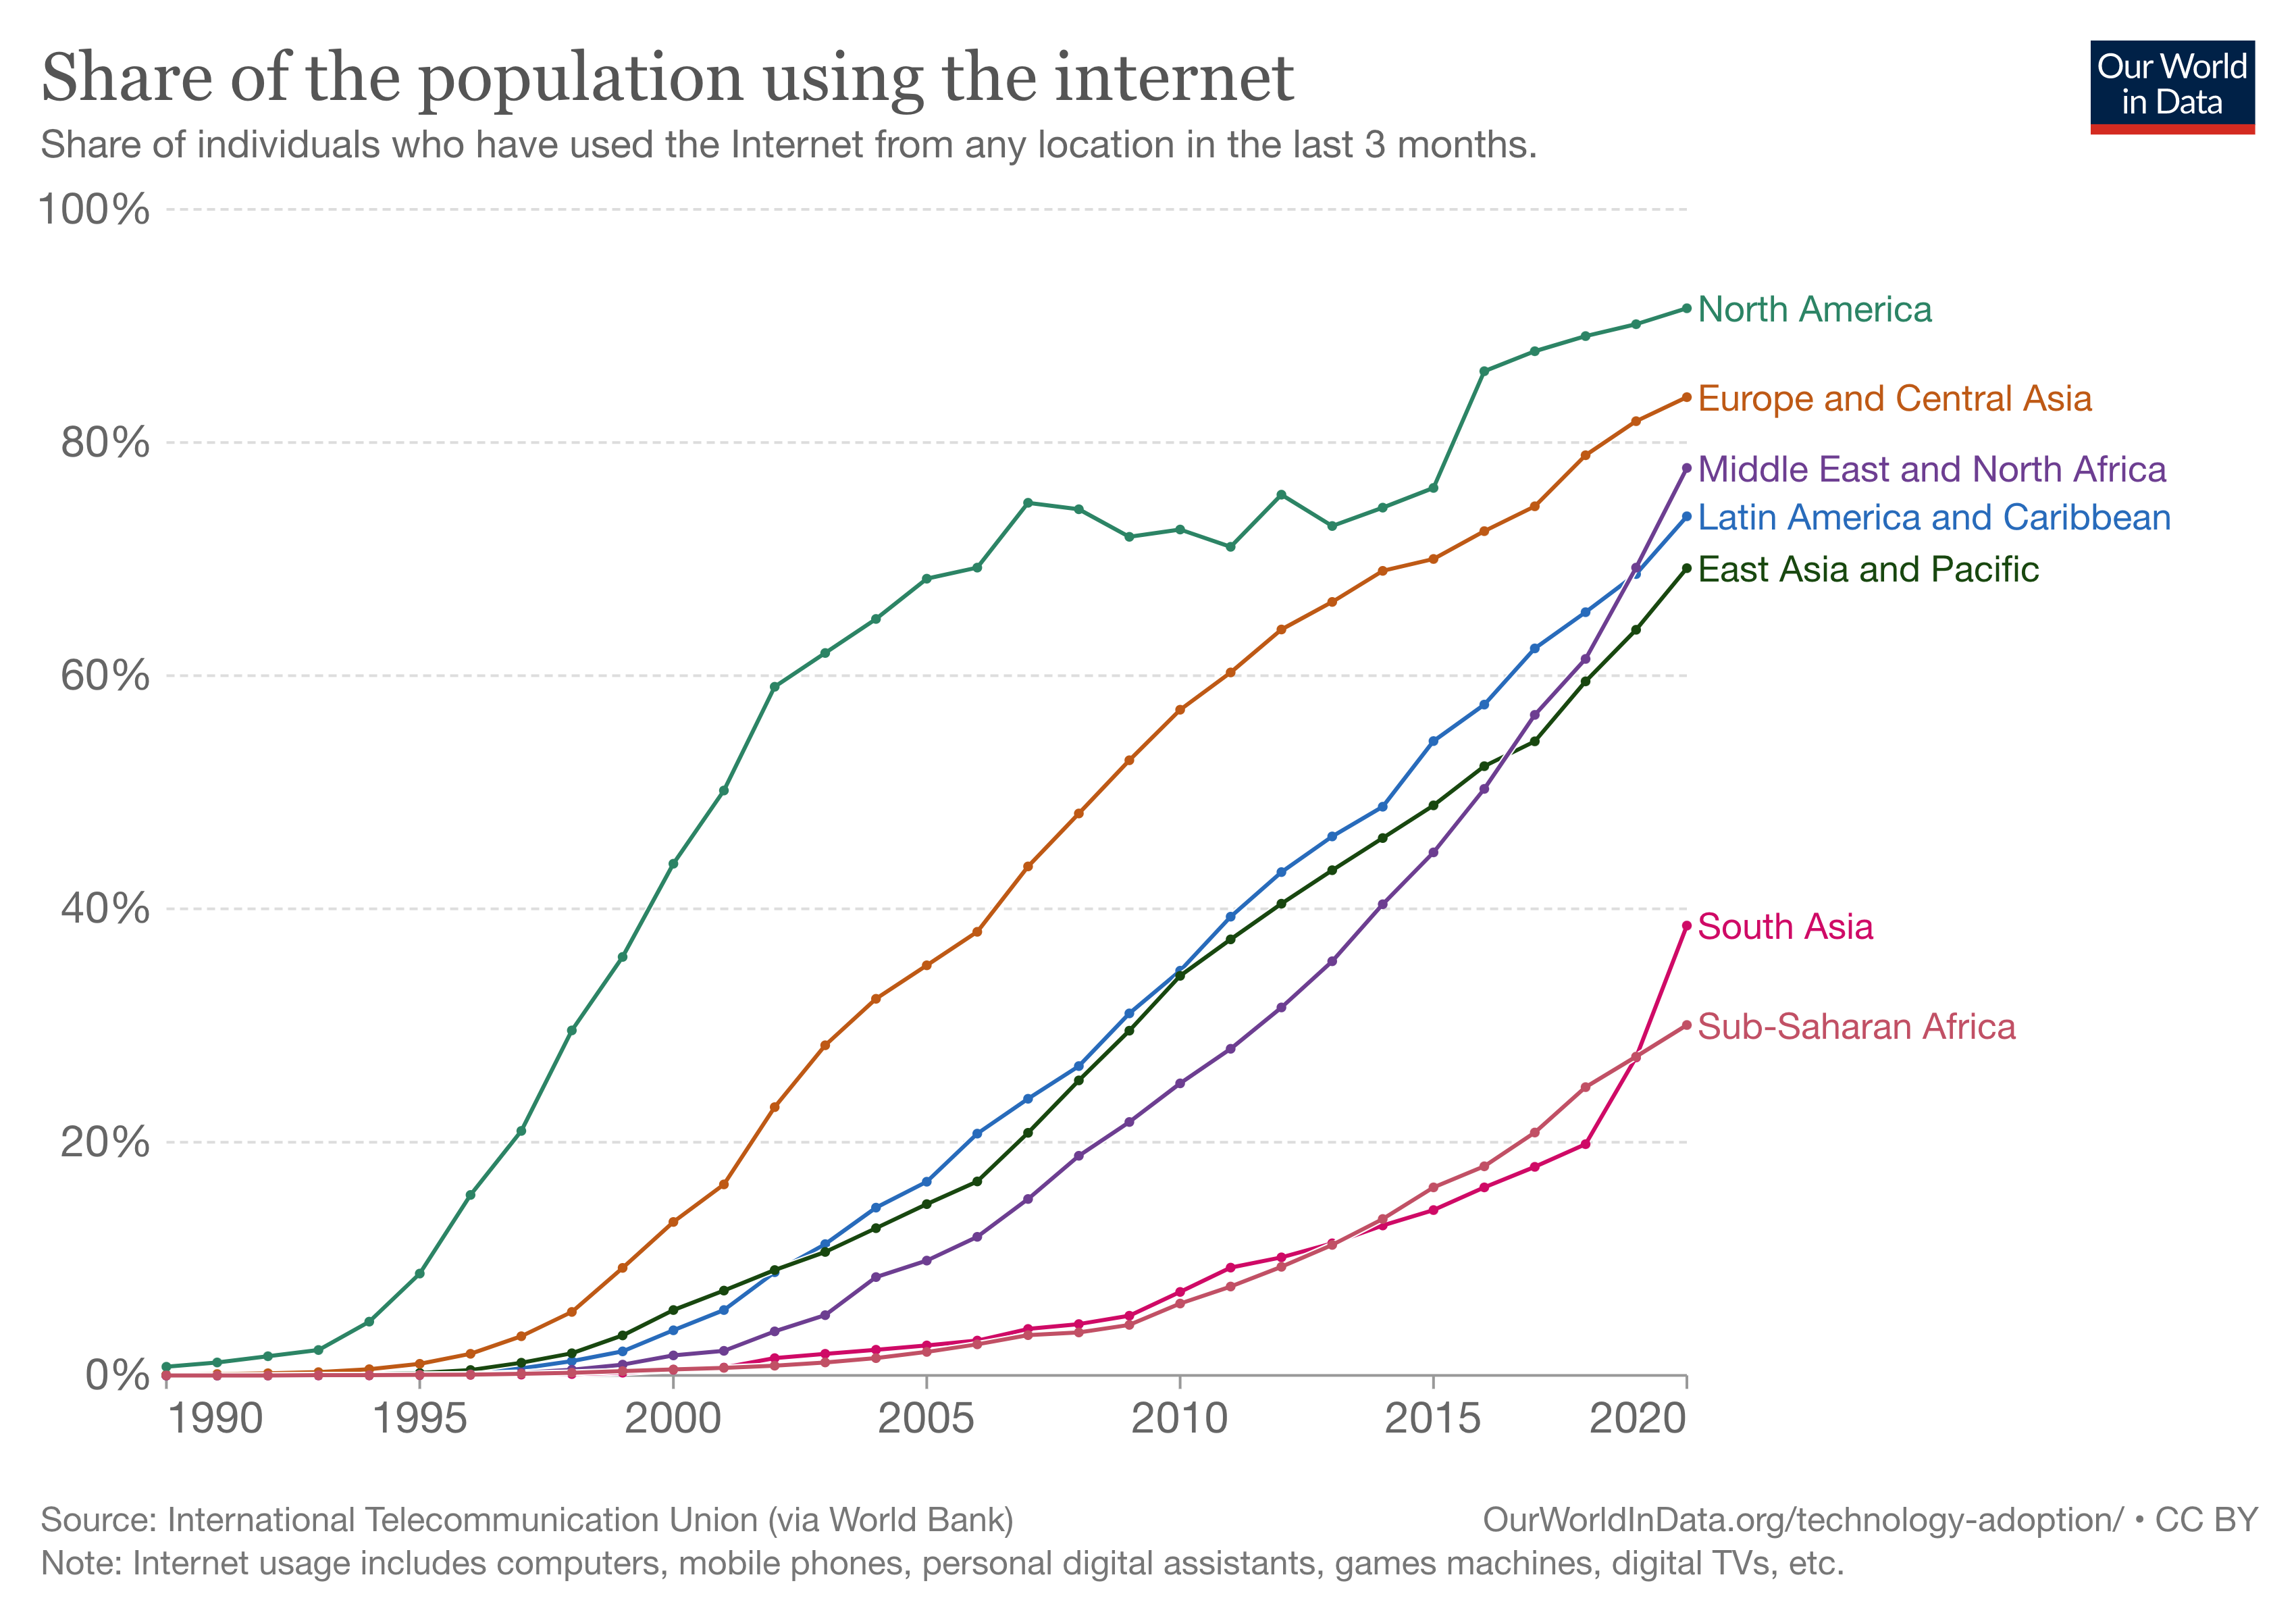
\includegraphics[width=0.8\textwidth]{koriscenje-interneta-po-godinama.png}
        \caption{Коришћење интернета током година}
        \label{slike:koriscenjeInterneta}
        \end{figure}
        
        Под компјутерским криминалом (познатим и као сајбер криминал, високотехнолошки криминал)  у најширем смислу подразумевају се кривична дела према кривичном закону националне државе, у којој су на било који начин укључени рачунарски системи и мреже.

        Главни циљ истраге сајбер криминала је, као и у случају класичног криминала, изградити за правосудне органе необорив, или чврст доказ, или доказ за ослобађање осумњиченог, или праведно санкционисање учињеног дела.
        Дигитални докази могу бити у форми коју генерише сам систем као производ рада рачунарског система (системски логови) и докази који су ускладиштени на рачунарском систему, као на пример база података корисника.
        Успешно сузбијање сајбер криминала подразумева стални развој дигиталне форензике. 
        
        Чињеничко стање у области сајбер криминала је следеће:
        \begin{enumerate}
            \item готово да не постоји ниједна већа организација на свету која није претрпела компромитовање својих система од стране нападача;
            \item већина аутсорсованих (енг. outsourced) програма се прави са бекдоровима (енг. backdoor), што може нападачу да омогући упад у систем;
            \item системи за детекцију напада на систем (енг. intrusion detection system - IDS) и антивируси нису решили безбедносне проблеме;
            \item постоји велики број умрежених рачунара (тзв. ботнет мрежа) намењених дистрибуцији нелегалних садржаја или пиратерије.
        \end{enumerate}
        На основу светских статистика може се рећи да је тренутно у свету од криминала процентуално најдоминантнији сајбер криминал. С озбиром на његов динамичан пораст и његових нових појавних облика, од дигиталне форензике се очекује да испрати све технолошке промене у информатици како би се што ефикасније суочила са изазовима које сајбер криминал доноси. Зато је бављење дигитално форензичким процесима постало незаобилазна дисциплина, када је реч о откривању недозвољених дигиталних активности и рачунарских инцидената.

        Колику важност има форензички одговор и колико је он осетљив, можда је и најсликовитији опис о потрази за дигиталним подацима дала Селиа Фридман\cite{fridmanCitat}:
        \begin{quote}
        “Сви подаци остављају траг. Потрага за подацима оставља траг. Брисање података оставља траг. Одсуство података под одређеним околностима може да остави најјаснији траг од свих.”
        \end{quote}
        
	\section{Типови сајбер криминала}
	\label{sec:TipoviVisKri}
	Када се спомену типови сајбер криминала (високотехнолошког
	криминала), онда се говори о активностима на основу којих је извршен напад заједно са различитим облицима техничких и информационих помагала. То могу бити различити хардверски уређаји или софтверска решења, која напад могу да олакшају наносећи штету физичким или правним лицима. \newline
	Професор Роналд Стандлер сајбер криминал према облику, односно врсти кривичног дела дели у три категорије: 1) неауторизовано коришћење рачунара, 2) стварање и дистрибуција штетних рачунарских програма, 3) узнемиравање и ухођење у сајбер простору. \newline
	Типови сајбер криминала, наведени у материјалу за “радионицу” о криминалу на мрежи са Десетог конгреса УН су наведени кроз дефиниције у ужем и ширем смислу:
	\begin{enumerate}
		\item Сајбер криминал у ужем смислу представља свако илегално понашање обављено електронским путем усмерено ка безбедности рачунарских система и подацима које они обрађују;
		\item Сајбер криминал у ширем смислу (криминал везан за рачунарску технологију) је свако илегално понашање обављено помоћу или у вези са рачунарским системом или рачунарском мрежом, укључујући и такве активности као што су илегално поседовање и/или нуђење и дистрибуција информација помоћу рачунарског система или рачунарске мреже. Наравно, највећи проблем приликом дефинисања овог термина представља разлика у законској регулативи у већини земаља.
	\end{enumerate}
	
	У истом документу наводе се и конкретни облици компјутерског криминалитета. То су:
	\begin{enumerate}
		\item неовлашћен приступ (упад) рачунарском систему или мрежи (онеспособљавање заштитних мера на систему или мрежи);
		\item оштећење рачунарских података или програма;
		\item рачунарска саботажа;
		\item неовлашћено пресретање комуникација у компјутерским системима и мрежама;
		\item рачунарска шпијунажа.
	\end{enumerate}
	Такође зависно од типа учињених дела сајбер криминал може имати политичку или економску позадину. \newline
	
	Према приказаним различитим категоријама ове врсте криминала могу се уочити различити интереси које мотивишу људе да почине законом забрањене радње. У пракси наравно постоје и случајеви када је у питању радозналост, самодоказивање или хвалисавост пред другим лицима. Зато се никада не може са сигурношћу говорити о јединственом профилу учинилаца рачунарског криминала, јер се они сврставају у различите категорије према појавним облицима дела која чине, али и према мотивима, који их покрећу у вршењу криминалних активности. \newline
	Учиниоци дела високотехнолошког криминала могли би се поделити на две групе:
	\begin{enumerate}
		\item злонамерне учиниоце, који могу да делују ради остварења имовинске користи, или само у циљу наношења штете или освете;
		\item учиниоце који нису мотивисани ни остварењем користи, нити проузроковањем штетних последица, већ једноставно траже задовољство у неовлашћеном продирању у неки добро обезбеђен информациони систем из забаве.
	\end{enumerate}

	\section{Примери из праксе}
	\label{sec:Primeriizprakse}
	Развој технологије и интернета, и њихова растућа улога у свакодневном животу људи довели су до раста сајбер криминала који се од ситних превара развио у злочине који наносе штету на глобалном нивоу. Последње две деценије обележили су многобројни случајеви високотехнолошког криминала великих размера. \newline
	Владимир Левин, софтверски инжењер из Петрограда, је након осамнаест упада у систем Citybank-а украо преко 10 милиона долара. Следеће године био је ухапшен и осуђен на 36 месеци затвора и новчану казну од 250.000 долара. \newline
	Први масовни напад десио се 1998. године, то је био „црв“ под називом Морис. Црв је самореплицирајући програм који уништава податке на рачунарима и шири се самостално по мрежи. За овај напад био је одговоран Роберт Тапан Морис.\newline
	Шеснаестогодишњак Џонатан Џозеф Џејмс је 1999. године извршио упад на Агенцију Министарства Одбране. Добио је приступ подацима као што су електронска пошта, корисничка имена и шифре запослених. Такође је упао и у НАСА рачунаре и украо програм вредан 1.7 милиона долара. Као последица тога НАСА је била принуђена да привремено искључи своје рачунарске системе, чиме је проузрокована велика финансијска штета. \newline
	До сада најопаснији црв јавио се 2003. године, који је у року од десет минута заразио 90 \% рачунарских система на планети који нису имали адекватну заштиту. Лондонски Market Intelligence  проценио је штету коју је овај црв изазвао на око 1.2 милијарде долара. \newline
	Појава електронског банкарства донела је нови талас сајбер криминала. Zeus је програм који се први пут појавио 2007. године, служи за крађу банкарских информација преко интернет претаживача. У то време јавила се и украјинска криминална организација која је 2009. у Румунији израђивала фалскификате кредитних картица којима је куповала злато које је касније користила за прање новца. \newline
	Познат случај је AshleyMadison.com из 2015. Канадски сајт за упознавање нападачи су користили да би набавили податке из целе базе корисника тог сајта. Свим корисницима, који су имали профиле са сликама, видео материјалима и чет комуникацијом, били су украдени подаци и објављени на Underground порталу и Dark Web-у. \newline
	Такође у 2015. години десио се авионски инцидент, који је проузрокован хакерским нападом на мобилни телефон. Уз помоћ одређеног програма нападачи су довели до експлозије телефона. \newline
	
	Следећа табела\cite{tabelaStete} приказује штета нанесену сајбер криминалом 2017. године по државама, у милијардама америчких долара: 
	\begin{table}[h!]
		\centering
		\begin{tabular}{|l|l|}
			\hline
			Државе & Штета \\ \hline
			Кина & 66.3 \\ \hline
			Бразил & 22.5 \\ \hline
			Америка & 19.4 \\ \hline
			Индија & 18.5 \\ \hline
			Мексико & 7.7 \\ \hline
			Француска & 7.1 \\
			\hline
		\end{tabular}
	\end{table}
	\section{Мере заштите}
	\label{sec:MereZastite}
	Уколико знамо да се свакодневница све брже и брже одвија и да се технологија дословно развија из дана у дан, неодговорно је сматрати да је безбедност искључена из опсега развоја који за циљ поред свих других има и онај део наше стварности који се односи на дестибилизацију система и опасности од сајбер напада\cite{semZastita}. Сајбер напади су све учесталији и у тренутку писања овог текста се десило више од 21 милиона напада у току овог дана\cite{brojNapada}. Али свест о опасности сајбер крими\-нала није довољно проширена и то представља један од главних пробле\-ма. Велике компаније јесу углавном мете сајбер напада, али то не значи да мале и средње компаније, као ни појединци, нису угрожени. Напротив, управо због слабијих мера заштита наведене категорије постају чешће мете напада. \newline
   	Наравно, ниједан систем није 100 \% сигуран јер сваки има своје слабо\-сти у виду рањивости у безбедоносним подешавањима на систему и
	злоупо\-треби функција програма. Анализа рањивости система која се обавља у комбинацији са дигиталном форензиком је јако значајна са
	станови\-шта заштите  да би организације могле да знају који су 
	пропусти присутни на системима, колико је тешко нападачу да их искористи и какве би последице могли да изазову. Безбедност на систе\-мима је добро описана кроз мото Ерис Соле-а: "Превенција је идеална, али је детекција обавезна"\cite{EricCole}. Већина организација заштиту на својим системима фокусира\-ју на превенцији, али не и на детектовању злона\-мерних активности. На пример, већина компанија на својим системима има инсталиране firewall-ове који делују превентивно. При томе се јављају два проблема. Први је тај да организација не може да спречи комплетан саобраћај, што на неки начин отвара могућност за потенци\-јални напад. Ту се јавља и један важан изазов свакој организацији да нађе баланс између безбедности, функционалности и проточности. И други проблем лежи у чињеници да нису сви превентивни механизми прилагођени или исправно конфигурисани па самим тим пружају мини\-малну заштиту. На пример антивируси не пружају потпуну заститу из разлога што раде на основу базе у којој имају информације о малициозним програми\-ма, али чим уђе у систем неки сасвим нов малициозни програм, антивирус га неће детектовати. Заштита се пости\-же непрекидним циклусом откривања слабости и њеним исправљањем. Само уколико постоји јасан став о разумевању безбедности рачунар\-ских система у оквиру организације и план да се безбедносни ризици смање, могу се превазићи безбедносни проблеми. 
	Превентивне методе које се могу применити јесу\cite{zastita1}\cite{zastita2}:
	\begin{enumerate}
		\item редовно ажурирање оперативног система и антивирусног софтвера
		\item опрезност и одговорност запослених или нас појединаца(на пример не отварати садржину мејла ако долази од непознатог пошиљаоца)
		\item спровођење редовних обука из домена сајбер безбедности 
		\item креирање профила за приступ, како би запослени приступали само оним деловима система који су неопходни за посао који обављају 
		\item креирање процедура за поступање у случајевима напада на инфор\-мационе систем компаније и обезбеђивање континуитета пословања 
		\item коришћење комплексних лозинки које садрже велики број измеша\-них слова, бројева и знакова, додатно могу се користити лозинке које истичу 			
		\item проактивно детектовање упада на систем коришћењем мамаца ханипотова({\em енг. Honeypot})\cite{hanipot} који симулирају рањиве сервисе система са циљем хватања нападача 
		\item употреба анализе рањивости 
	\end{enumerate}
	
	Ово су само неке од превентивних мера које се могу преузети. Важно је истаћи да не постоји начин да се рачунарски системи правилно заштите, уколико се не зна против чега је усмерена заштита.
	\section{Закључак}
	\label{sec:Zakljucak}
	Шта даље очекивати од развоја како безбедоносних мера, тако и технологија помоћу којих се могу извршавати сајбер напади? Једно је сигурно, број сајбер напада ће се увећати у будућности и много више утицати на нас како се технологија буде све више интегрисала у нашим свакодневним животима. То је само једна од многих претњи којима се нападачи користе. Технологија на претњу сајбер криминалу одговара развојем сигурносних система које би правила вештачка интелигенција тако што би учила на претходним примерима малициозних напада, научила да их детектује и у крајњем случају и уклони\cite{AIsecurity}. Али са друге стране ту лежи и опасност примене вештачке интелигенције у развоју малициозних програма. Оно што ми можемо да предузмемо у нашој будућности је да поштујемо мере заштите и да будемо опрезни. 

\newpage
    \addcontentsline{toc}{section}{Литература}
    \appendix

    \bibliography{seminarski} 
    \bibliographystyle{plain}

    \begin{thebibliography}{9}

    \bibitem{fridmanCitat}C. S. Friedman, \emph{This Alien Shore}, DAW BOOKS, INC, New York 1998.

    \bibitem{knjigaDigiForenzika}В. Кораћ, Д. Прља, А. Дилигенски \emph{Дигитална Форензика}, Београд 2016.

    \bibitem{tabelaStete}Табела штете нанесене сајбер криминалом, https://www.statista.com/statistics/799875/countries-with-the-largest-losses-through-cybercrime/
    
    \bibitem{semZastita}Сајбер тероризам као окидач све интензивније потребе за безбедност система од опасности које долазе са интернет, Сандра Клисарић, 14.04.2021
	  
    \bibitem{brojNapada} Сајт који приказује број сајбер напада у току једног дана https://threatmap.checkpoint.com/
	  
    \bibitem{EricCole}Eric Cole, \emph{How to secure your company, Computerworld} 11.06.2016 
	  
    \bibitem{zastita1}Превенција сајбер напада https://www.cert.rs/files/shares/Prevencija%20i%20za%C5%A1tita%20malih%20i\%20srednjih\%20preduze\%C4\%87a\%20od\%20sajber\%20napada.pdf
	  
    \bibitem{zastita2}Врсте сајбер напада https://www.cert.rs/files/shares/3.\%20Vrste-sajber-napada-ratel-cert.pdf
	  
    \bibitem{hanipot}Ханипот и где се користи https://www.kaspersky.com/resource-center/threats/what-is-a-honeypot
	  
    \bibitem{AIsecurity} Вештачка интелигенција у сигурносним системима https://www.vectra.ai/learning/ai-security2
    
    \end{thebibliography}
	
    \appendix

\end{document}